%
% teil1.tex -- Beispiel-File für das Paper
%
% (c) 2020 Prof Dr Andreas Müller, Hochschule Rapperswil
%
\section{Spiegelung}
\rhead{Spiegelung}

Die Spiegelung ist eine grundlegende, geometrische Operation, aus welcher man weitere, wie beispielsweise die später beschriebene Rotation, ableiten kann. Da die geometrische Algebra für geometrische Anwendungen ausgelegt ist, sollte die Spiegelung auch eine einfache, praktische Formulierung besitzen.
\begin{figure}
	\centering
	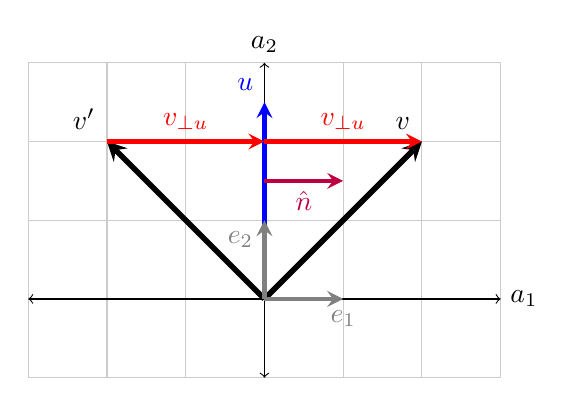
\begin{tikzpicture}
		\draw[thin,gray!40] (-3,-1) grid (3,3);
		\draw[<->] (-3,0)--(3,0) node[right]{$a_1$};
		\draw[<->] (0,-1)--(0,3) node[above]{$a_2$};
		\draw[line width=2pt,black,-stealth](0,0)--(2,2) node[anchor=south east]{$\boldsymbol{v}$};
		\draw[line width=1.5pt,blue,-stealth](0,0)--(0,2.5) node[anchor=south east]{$\boldsymbol{u}$};
		\draw[line width=2pt,black,-stealth](0,0)--(-2,2) node[anchor=south east]{$\boldsymbol{v'}$};
		\draw[line width=1.5pt,gray,-stealth](0,0)--(1,0) node[anchor=north]{$\boldsymbol{e_1}$};
		\draw[line width=1.5pt,gray,-stealth](0,0)--(0,1) node[anchor=north east]{$\boldsymbol{e_2}$};
		\draw[line width=1.5pt,red,-stealth](0,2)--(2,2) node[xshift=-1cm, yshift=
		0.25cm]{$\boldsymbol{v_{\perp u}}$};
		\draw[line width=1.5pt,red,-stealth](-2,2)--(0,2) node[xshift=-1cm, yshift=
		0.25cm]{$\boldsymbol{v_{\perp u}}$};
		\draw[line width=1.5pt,purple,-stealth](0,1.5)--(1,1.5) node[xshift=-0.5cm, yshift=-0.25cm]{$\boldsymbol{\hat{n}}$};
	\end{tikzpicture}
	\caption{Spiegelung des Vektors \textbf{v} an Spiegelachse bzw. Vektor \textbf{u}}
	\label{BildSpiegelung}
\end{figure}

\subsection{Linearen Algebra}
Aus der linearen Algebra ist bekannt, dass man eine Spiegelung an einer Ebene wie folgt beschreiben kann.
\begin{definition}
	Die Spiegelungsgleichung in der linearen Algebra mit dem Normalenvektor $\mathbf{\hat{n}}$ zur Spiegelebene ist
	\begin{equation} \label{RefLinAlg}
		\mathbf{v^{'}} = \mathbf{v} - 2 \cdot \mathbf{v_{\parallel \hat{n}}} = \mathbf{v} - 2 \cdot \mathbf{v_{\perp u}}.
	\end{equation}
	Per Definition sind $\mathbf{v_{\parallel \hat{n}}} = \mathbf{v_{\perp u}}$. In der geometrischen Algebra verwenden wir aber in den Formeln Vektoren, welche Spiegelachsen, nicht Spiegelebenen, repräsentieren.
\end{definition}
Es scheint für diese Formel aber umständlich zu sein, weitere Spiegelungen mit weiteren Spiegelebenen anzufügen. Man kann diese Abbildung aber auch als Matrix schreiben. Sei $\mathbf{\hat{n}}$ ein Normalenvektor auf die Spiegelungs-Achse bzw. -Ebene, also $\mathbf{\hat{n}}\perp \mathbf{u}$, und sei ausserdem normiert $|\mathbf{\hat{n}}| = 1$, dann kann man die Spiegelung durch die Matrix
\begin{align}
	S = E - 2\dfrac{1}{|\mathbf{n}|^2}\mathbf{nn}^t
\end{align}
beschrieben werden. In der zweiten und dritten Dimension ergibt die Berechnung
\begin{align} \label{Spiegelmatrizen}
	S_2 = \begin{pmatrix}
		1-2n_1^2 & -2n_1n_2 \\
		-2n_1n_2 & 1-2n_2^2
	\end{pmatrix} \quad
	S_3 = \begin{pmatrix}
		1-2n_1^2 & -2n_1n_2 & -2n_1n_3\\
		-2n_1n_2 & 1-2n_2^2 & -2n_2n_3\\
		-2n_1n_3 & -2n_2n_3 & 1-2n_3^2\\
	\end{pmatrix}.
\end{align}
Diese Spiegelmatrizen gehören der orthogonalen Matrizengruppe $S\in \text{O}(n)$ an. Die Matrizengruppe $\text{O}(n)$ haben die Eigenschaft $S^t S = E$, was bedeutet, dass die Länge und Winkel bei der Abbildung beibehalten bleiben. Zusätzlich sind die Spiegelmatrizen symmetrisch, es gilt $S^t = S$. Somit liefert zweimal dieselbe Spiegelung wieder die identische Abbildung, wie man aus
\begin{align}
	S^t S = S^2 = E
\end{align}
schliessen kann.

\subsection{Geometrische Algebra}
Um die folgenden Formeln zu verstehen, definieren wir zuerst die Inverse eines Vektors, welche in dieser Form nicht in der linearen Algebra nicht existiert.
\begin{definition}
	Die Inverse eines Vektors wird definiert als
	\begin{align}
		\mathbf{u}^{-1} = \dfrac{\mathbf{u}}{|\mathbf{u}|^2} \Rightarrow \mathbf{uu}^{-1} = \dfrac{\mathbf{u}^2}{|\mathbf{u}|^2} = 1.
	\end{align}
	Wie schon aus anderen algebraischen Strukturen bekannt, ergibt ein Element, hier $\mathbf{u}$, multipliziert mit dessen Inversen, hier $\mathbf{u}^{-1}$, das neutrale Element der Struktur, hier 1.
\end{definition}
Die geometrische Algebra leitet aus der obigen Formel \eqref{RefLinAlg} für eine Spiegelung eine einfache und intuitive Form her, welche auch für weitere Operationen erweitert werden kann.
\begin{definition}
	Die Spiegelungsgleichung in der geometrischen Algebra mit der Spiegelachse $\mathbf{u}$ ist definiert als
	\begin{align}\label{RefGA}
		\mathbf{v}' = \mathbf{uvu}^{-1}
	\end{align}
\end{definition}

verwendet man für $\mathbf{u}$ nur einen Einheitsvektor $\mathbf{\hat{u}}$, welcher die Länge 1 besitzt, wird die Gleichung zu
\begin{align}
	\mathbf{v'} = \mathbf{\hat{u}v\hat{u}}
\end{align}
vereinfacht. Im Gegensatz zu den Abbildungen in der linearen Algebra, welche in jeder anderen Dimension, durch andere Matrizen \eqref{Spiegelmatrizen} beschrieben werden müssen, ist es in der geometrischen Algebra immer der gleiche Vorgehensweise. Zudem ist diese kompakte Schreibweise in der linearen Algebra nicht möglich, da bis auf das Vektorprodukt in der dritten Dimension keine Multiplikation von Vektoren definiert ist. 